\documentclass[11pt,a4paper]{article}

\usepackage[T1]{fontenc}
\usepackage[utf8]{inputenc}
\usepackage[english,brazil]{babel}
\usepackage[a4paper,margin=2.5cm]{geometry}
\usepackage{lmodern}
\usepackage{microtype}
\usepackage{amsmath}
\usepackage{graphicx}
\usepackage{booktabs}
\usepackage{tabularx}
\usepackage{float}
\usepackage{xcolor}
\usepackage{csquotes}
\usepackage{caption}
\usepackage{hyperref}

\graphicspath{{./}{./images/}}

\definecolor{linkblue}{RGB}{30,75,180}
\hypersetup{
    colorlinks=true,
    linkcolor=linkblue,
    urlcolor=linkblue,
    citecolor=linkblue,
    pdftitle={Projeto Experimental de Integração e Validação de Sensores para Navegação Relativa em Ambiente sem GPS},
    pdfauthor={Gabriel Holsback Dantas; Rafael de Queiroz Lavoyer}
}
\captionsetup{font=small,labelfont=bf}
\setlength{\parindent}{1.25cm}
\setlength{\parskip}{0pt}
\setcounter{topnumber}{3}
\setcounter{totalnumber}{5}
\renewcommand{\topfraction}{0.9}
\renewcommand{\textfraction}{0.05}
\renewcommand{\floatpagefraction}{0.8}

\usepackage[
    backend=biber,
    style=authoryear,
    sorting=nyt,
    maxcitenames=2,
    maxbibnames=99
]{biblatex}
\addbibresource{main.bib}
\AtBeginBibliography{\small}

\title{\textbf{Projeto Experimental de Integração e Validação de Sensores para Navegação Relativa em Ambiente sem GPS}}
\author{Gabriel Holsback Dantas \quad Rafael de Queiroz Lavoyer\\[0.4em]
\small Curso de Engenharia da Computação, Centro Universitário de Brasília (CEUB)\\
\small \href{mailto:holsback@sempreceub.com}{holsback@sempreceub.com} \quad
\href{mailto:rafael.lavoyer@sempreceub.com}{rafael.lavoyer@sempreceub.com}}
\date{}

\begin{document}

\maketitle

\input{sections/abstract}
\chapter{Introdução}
\label{cap:introducao}

O mapeamento tridimensional de ambientes confinados é relevante para inspeção, documentação e exploração de locais onde a presença humana pode ser arriscada ou operacionalmente custosa. Cavernas, galerias, áreas industriais internas e regiões de difícil acesso têm em comum a baixa disponibilidade de infraestrutura externa de posicionamento. Em particular, sistemas baseados em GPS tendem a apresentar indisponibilidade ou degradação severa nesses cenários, exigindo métodos de localização relativa baseados em sensores embarcados \cite{thrun2005probabilistic,beardMcLain2012}.

Uma solução direta seria integrar as acelerações medidas por uma Unidade de Medição Inercial (IMU) para obter velocidade e posição. Entretanto, essa abordagem isolada é limitada: pequenos vieses, ruídos de quantização e erros de atitude são integrados ao longo do tempo, produzindo deriva crescente na estimativa de posição \cite{tittertonWeston2004,groves2013principles,farrell2008aided}. Por outro lado, sensores ópticos de fluxo medem deslocamentos relativos da superfície observada entre quadros consecutivos, fornecendo uma fonte direta de odometria no plano observado, especialmente útil em navegação indoor e em ambientes sem GPS \cite{lucasKanade1981,pixart2017pmw3901}.

Este trabalho adota uma arquitetura híbrida. O sensor óptico de fluxo é tratado como fonte primária de deslocamento no plano horizontal, com correção de escala pela altura medida por um sensor ToF. A IMU complementa essa estimativa ao fornecer atitude do drone e ao preencher pequenos intervalos nos quais o sensor óptico não registra evento de movimento. O LiDAR 2D, por sua vez, fornece distância, ângulo e intensidade de retorno para cada ponto de varredura. Com a posição e a atitude estimadas, cada ponto LiDAR é transformado do referencial local do sensor para o referencial global, resultando em uma nuvem de pontos tridimensional.

\section{Problema de pesquisa}

O problema investigado pode ser resumido na seguinte pergunta: como estimar a posição relativa de uma plataforma móvel em ambiente sem GPS e usar essa pose para transformar medições LiDAR em uma nuvem de pontos global coerente? A resposta proposta combina três fontes de informação com papéis distintos: fluxo óptico para deslocamento horizontal, IMU para orientação e propagação em intervalos sem medição óptica, e LiDAR para geometria do ambiente.

\section{Objetivos}

O objetivo geral deste trabalho é desenvolver e documentar um fluxo de aquisição e processamento capaz de estimar a localização relativa de um drone em ambiente sem GPS e gerar uma nuvem de pontos tridimensional no referencial global a partir da combinação de sensor óptico, IMU e LiDAR.

Os objetivos específicos são:

\begin{itemize}
    \item Integrar em uma plataforma embarcada sensores de fluxo óptico, ToF, IMU e LiDAR, registrando os dados em formato sincronizado por timestamp.
    \item Converter e filtrar os sinais inerciais para estimar atitude e aceleração linear no referencial global.
    \item Estimar a trajetória no plano $XY$ usando fluxo óptico como fonte primária e integração inercial apenas nos intervalos sem eventos do sensor óptico.
    \item Processar os pontos LiDAR com filtros físicos e estatísticos, convertendo distância e ângulo para coordenadas locais.
    \item Transformar a nuvem local do LiDAR para o referencial global usando posição, atitude e hipóteses de montagem do sensor.
    \item Identificar limitações experimentais e parâmetros que ainda dependem de calibração final.
\end{itemize}

\section{Contribuições}

As principais contribuições deste trabalho são:

\begin{itemize}
    \item Definição de uma arquitetura de sensoriamento para navegação relativa em ambiente sem GPS, usando fluxo óptico como odometria primária e IMU como apoio inercial.
    \item Definição de um fluxo de processamento para conversão de unidades, calibração de viés do giroscópio, filtragem Butterworth, estimação de atitude por Madgwick e fusão de posição no plano $XY$.
    \item Definição de um fluxo de geração de nuvem global que considera a rotação do LiDAR principal em torno do eixo $Y$ do drone e aplica filtros automáticos de intensidade, distância e continuidade de pose.
    \item Organização das hipóteses e limitações do experimento, especialmente a ausência de odometria vertical dedicada e a necessidade de validação da calibração extrínseca entre sensores.
\end{itemize}

\section{Organização do trabalho}

O Capítulo~\ref{cap:conceitos} apresenta os conceitos de sensores embarcados, navegação inercial, fluxo óptico, atitude, transformações de coordenadas e filtragem usados no projeto. O Capítulo~\ref{cap:metodologia} descreve a plataforma, os dados coletados e o método de processamento adotado. O Capítulo~\ref{cap:resultados_conclusao} apresenta a implementação, os resultados obtidos, as limitações e os trabalhos futuros.

\input{sections/concepts}
\input{sections/methodology}
\chapter{Conclusão}

Fringilla urna porttitor rhoncus dolor. Iaculis urna id volutpat lacus laoreet. Nullam non nisi est sit amet facilisis magna etiam. Ultrices vitae auctor eu augue. Cursus vitae congue mauris rhoncus aenean vel. Donec ultrices tincidunt arcu non. Id diam vel quam elementum pulvinar etiam non quam. Faucibus a pellentesque sit amet porttitor eget dolor. Tellus at urna condimentum mattis pellentesque. Ut sem viverra aliquet eget sit amet tellus cras adipiscing.

\section{Arquitetura do Projeto}

O sistema desenvolvido é composto por uma arquitetura modular integrada em uma plataforma móvel terrestre, com possibilidade de migração para plataforma aérea. A arquitetura pode ser descrita conforme a sequência de transformação de dados:

\begin{center}
LiDAR (sensor) $\rightarrow$ Corpo (drone) $\rightarrow$ Referencial Global
\end{center}

\subsection{Componentes Principais}

O sistema integra três sensores principais para aquisição de dados espaciais:

\begin{itemize}
    \item \textbf{Sensor LiDAR LD06:} Responsável pela medição de distância e ângulo, fornecendo pares (ângulo, distância) com resolução angular e intensidade do retorno, permitindo a geração da nuvem de pontos em 2D.
    
    \item \textbf{Unidades de Medição Inercial (IMU) — 2x MPU-6050:} Medem aceleração em três eixos (ax, ay, az) e velocidade angular (gx, gy, gz), viabilizando a estimação de atitude do drone e a derivação de posição inercial através de integrações sucessivas.
    
    \item \textbf{Microcontrolador Raspberry Pi Pico (RP2040):} Orquestra a leitura dos sensores, sincroniza os dados, aplica filtros de qualidade e registra o conjunto completo em cartão SD. Possui 264 KB de RAM, 2 MB de Flash e periféricos suficientes (2x UART, 2x I2C, 2x SPI) para gerenciar todos os sensores simultaneamente.
\end{itemize}

\subsection{Fluxo de Processamento}

O processamento ocorre em etapas sequenciais:

\begin{enumerate}
    \item \textbf{Aquisição:} Leitura simultânea das duas IMUs via I2C e do LiDAR via UART serial.
    \item \textbf{Filtragem:} Aplicação de filtro de intensidade mínima (223) para garantir qualidade dos dados LiDAR.
    \item \textbf{Sincronização Temporal:} Timestamping em microsegundos para correlacionar medições de sensores distintos.
    \item \textbf{Compensação Inercial:} Transformação de acelerações do referencial do corpo para o referencial global utilizando matrizes de rotação baseadas nos ângulos de Euler (roll, pitch, yaw).
    \item \textbf{Integração Numérica:} Cálculo de velocidade e posição pela dupla integração de aceleração (v = $\int$ a dt, s = $\int$ v dt).
    \item \textbf{Armazenamento:} Gravação contínua em cartão SD no formato CSV para posterior processamento e geração de nuvem de pontos.
\end{enumerate}

\subsection{Diagrama de Arquitetura}

\begin{figure}[H]
    \centering
    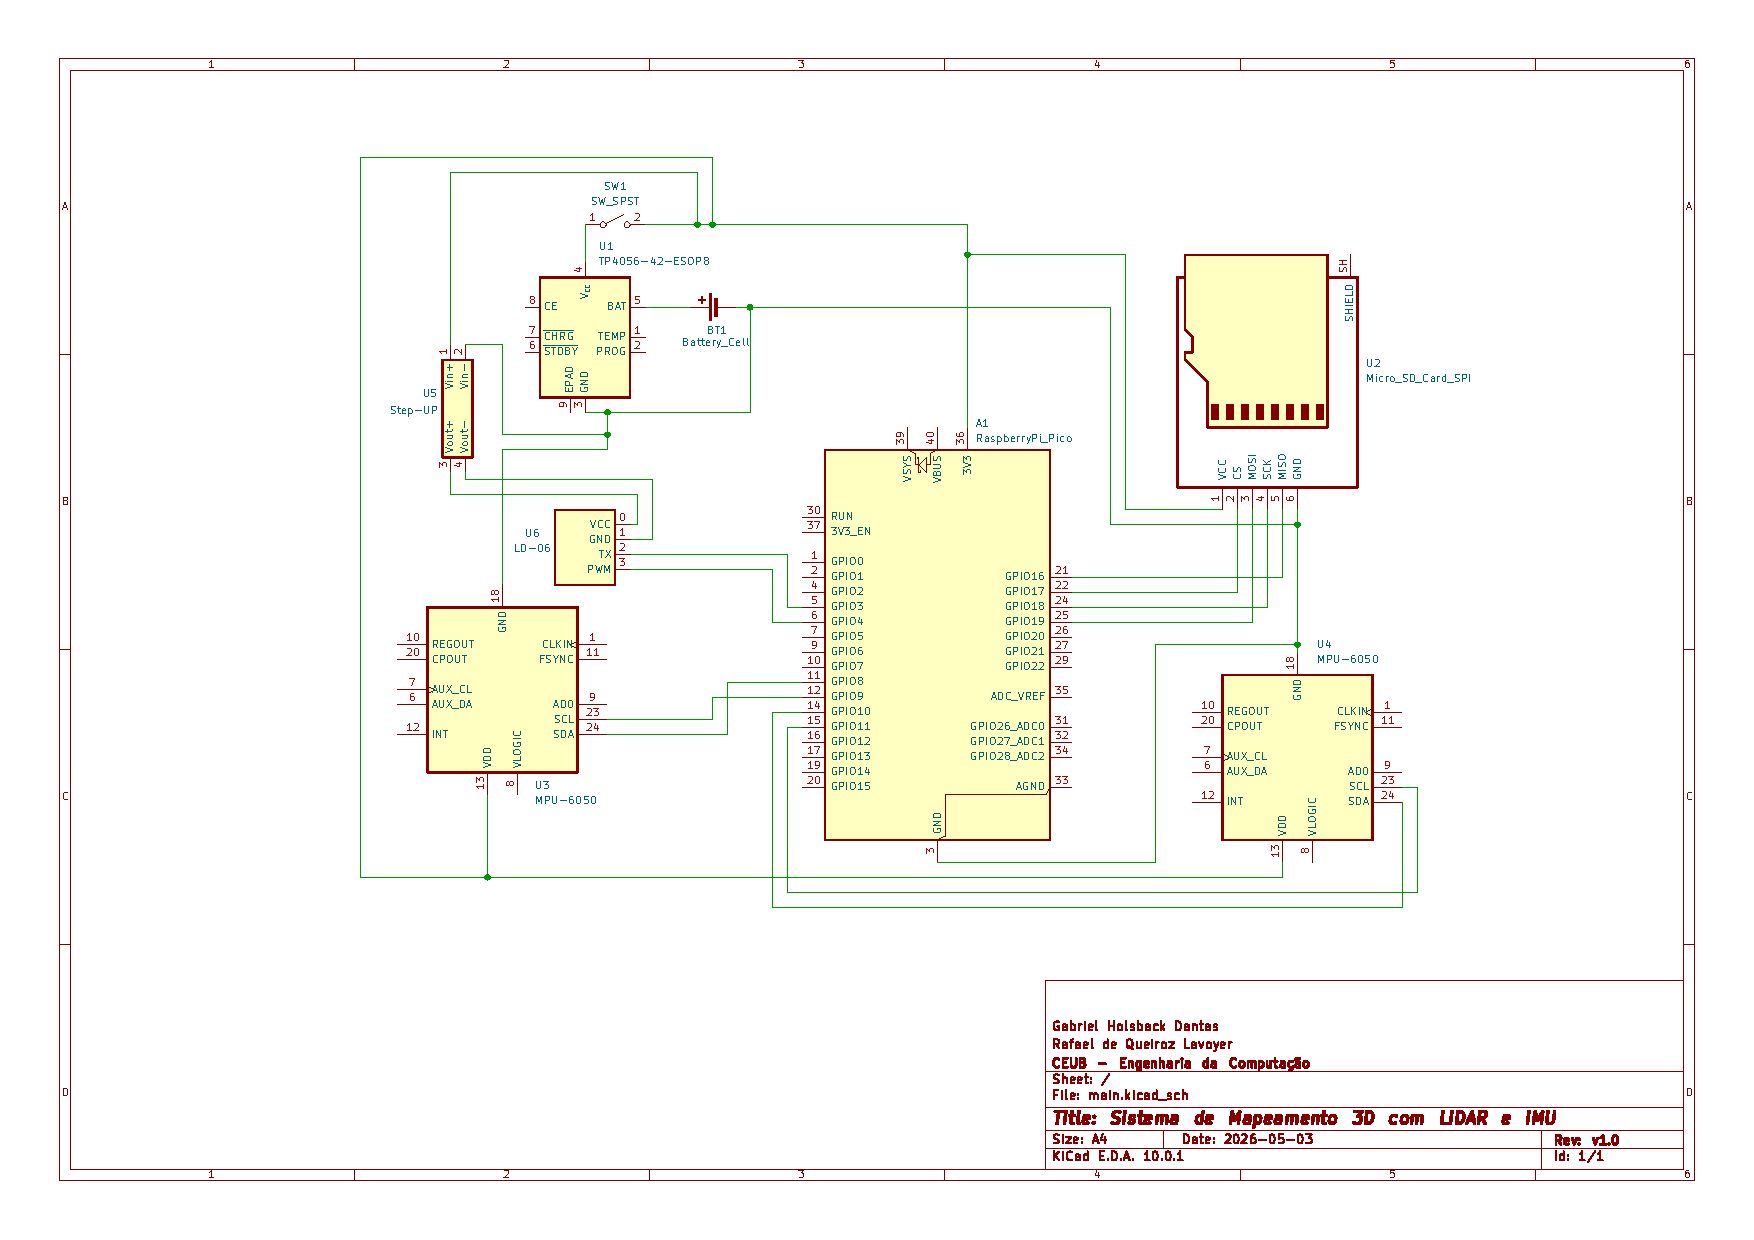
\includegraphics[width=0.8\textwidth]{Componentes}
    \caption{Diagrama esquemático da arquitetura de hardware do sistema de mapeamento 3D, mostrando a integração entre o Raspberry Pi Pico, sensores (LiDAR LD06 e IMUs MPU-6050), módulo de armazenamento (cartão SD) e plataforma móvel.}
    \label{fig:arquitetura_hardware}
\end{figure}

\section{Materiais Utilizados}

O projeto foi implementado com componentes específicos selecionados pela sua adequação aos requisitos de precisão, custo e integração:

\subsection{Componentes Eletrônicos}

\subsubsection{Microcontrolador}
\begin{itemize}
    \item \textbf{Componente:} Raspberry Pi Pico (RP2040)
    \item \textbf{Especificações:} Processador ARM Cortex-M0+ dual-core @ 125 MHz, 264 KB RAM, 2 MB Flash, 2x UART, 2x I2C, 2x SPI, 16x PWM, ADC
    \item \textbf{Função:} Controlar sensores, processar dados e gerenciar armazenamento em tempo real
\end{itemize}

\subsubsection{Sensores Inerciais}
\begin{itemize}
    \item \textbf{Componente:} MPU-6050 (Quantidade: 2 unidades)
    \item \textbf{Especificações:} Acelerómetro ±2g a ±16g, Giroscópio ±250°/s a ±2000°/s, Interface I2C
    \item \textbf{Função:} Medir aceleração (ax, ay, az) e velocidade angular (gx, gy, gz) para estimativa de atitude e posição inercial
\end{itemize}

\subsubsection{Sensor de Distância e Ângulo}
\begin{itemize}
    \item \textbf{Componente:} LiDAR LD06 (2D)
    \item \textbf{Especificações:} UART 230400 baud, Pacotes de 47 bytes com 12 pontos cada, Varredura 0° a 360°, Filtro de qualidade em intensidade ≥ 223
    \item \textbf{Função:} Medir distância e ângulo para geração de nuvem de pontos 2D
\end{itemize}

\subsubsection{Armazenamento}
\begin{itemize}
    \item \textbf{Componente:} Módulo Cartão SD
    \item \textbf{Especificações:} Interface SPI, Capacidade mínima de 16 GB
    \item \textbf{Função:} Registrar 15 variáveis de dados por ciclo em formato CSV
\end{itemize}

\subsection{Dados Coletados}

O sistema coleta um conjunto robusto de dados em cada ciclo de leitura:

\begin{table}[H]
    \centering
    \caption{Estrutura de dados coletados por ciclo}
    \begin{tabularx}{\textwidth}{l|l|X}
        \hline
        \textbf{Variável} & \textbf{Fonte} & \textbf{Descrição} \\
        \hline
        tempo\_us & Relógio & Timestamp em microsegundos \\
        ax1, ay1, az1 & IMU 1 & Aceleração nos 3 eixos (IMU 1) \\
        gx1, gy1, gz1 & IMU 1 & Velocidade angular nos 3 eixos (IMU 1) \\
        ax2, ay2, az2 & IMU 2 & Aceleração nos 3 eixos (IMU 2) \\
        gx2, gy2, gz2 & IMU 2 & Velocidade angular nos 3 eixos (IMU 2) \\
        angle & LiDAR & Ângulo da varredura LiDAR (0° a 360°) \\
        distance & LiDAR & Distância medida (unidades de 0.25 mm) \\
        intensity & LiDAR & Intensidade do retorno laser (0--255) \\
        \hline
    \end{tabularx}
    \label{tab:dados_coletados}
\end{table}

Os dados são armazenados em formato CSV, permitindo análise posterior e processamento para geração da nuvem de pontos com transformação completa de coordenadas.

\section{Dificuldades}

\section{Resultados obtidos}

\subsection{Interpretação dos resultados}

\section{Trabalhos futuros}

\subsection{Comunicação com o drone em cavernas}

\subsection{Navegação autônoma com os dados obtidos}




\printbibliography[title={Referências}]

\appendix
\section{Pipeline de processamento da IMU e do sensor óptico}
\label{ap:posicao}

O notebook complementar \path{imu_pipeline_flow_v2.ipynb} registra a etapa que converte as leituras inerciais, estima o viés dos giroscópios, filtra e combina as duas IMUs, calcula a atitude pelo filtro de Madgwick e acumula os incrementos do sensor óptico corrigidos pelo ToF. Seus produtos principais são a posição relativa e a atitude associadas aos instantes de aquisição do LiDAR.

O arquivo deve ser executado a partir da raiz do projeto, onde se encontram os dados de entrada. Parâmetros dependentes do ensaio, como janela de calibração, frequências de corte, faixa válida do ToF e convenção de eixos, estão concentrados nas células iniciais. As figuras intermediárias devem ser inspecionadas antes da exportação, especialmente para verificar saturação, orientação inicial e intervalos sem eventos ópticos.

\section{Processamento da nuvem de pontos global com LiDAR}
\label{ap:nuvem}

O notebook complementar \path{processamento_nuvem_lidar_global.ipynb} recebe a posição e a atitude associadas aos retornos LiDAR, aplica os critérios físicos e estatísticos, transforma os pontos para o referencial global relativo e exporta \path{nuvem_pontos_lidar_global.csv}. O mesmo material gera as visualizações \path{nuvem_global_3d.png} e \path{nuvem_global_2d.png} e calcula as amplitudes robustas usadas na comparação dimensional horizontal.

Em outra montagem, devem ser revisados a escala, a convenção angular e os parâmetros extrínsecos. Os valores identidade e nulo foram hipóteses exclusivas desta prova de conceito.


\end{document}
